\documentclass[letterpaper,11pt]{article}

\usepackage{latexsym}
\usepackage[empty]{fullpage}
\usepackage{titlesec}
\usepackage{marvosym}
\usepackage[usenames,dvipsnames]{color}
\usepackage{verbatim}
\usepackage{enumitem}
\usepackage[hidelinks]{hyperref}
\usepackage{fancyhdr}
\usepackage[english]{babel}
\usepackage{tabularx}
\usepackage{fontawesome5}
\usepackage{multicol}
\setlength{\multicolsep}{-3.0pt}
\setlength{\columnsep}{-1pt}
\input{glyphtounicode}

%new packages

\usepackage{fontenc}
\usepackage{amsmath}
\usepackage{amssymb}
\usepackage{graphicx}



%----------FONT OPTIONS----------

\pagestyle{fancy}
\fancyhf{} % clear all header and footer fields
\fancyfoot{}
\renewcommand{\headrulewidth}{0pt}
\renewcommand{\footrulewidth}{0pt}

% Adjust margins
\addtolength{\oddsidemargin}{-0.6in}
\addtolength{\evensidemargin}{-0.5in}
\addtolength{\textwidth}{1.19in}
\addtolength{\topmargin}{-.7in}
\addtolength{\textheight}{1.4in}

\urlstyle{same}

\raggedbottom
\raggedright
\setlength{\tabcolsep}{0in}

% Sections formatting
\titleformat{\section}{
  \vspace{-4pt}\scshape\raggedright\large\bfseries
}{}{0em}{}[\color{black}\titlerule \vspace{-5pt}]



% Ensure that generate pdf is machine readable/ATS parsable
\pdfgentounicode=1

%-------------------------
% Custom commands
\newcommand{\resumeItem}[1]{
  \item\small{
    {#1 \vspace{-2pt}}
  }
}

\newcommand{\classesList}[4]{
    \item\small{
        {#1 #2 #3 #4 \vspace{-2pt}}
  }
}

\newcommand{\resumeSubheading}[4]{
  \vspace{-2pt}\item
    \begin{tabular*}{1.0\textwidth}[t]{l@{\extracolsep{\fill}}r}
      \textbf{#1} & \textbf{\small #2} \\
      \textit{\small#3} & \textit{\small #4} \\
    \end{tabular*}\vspace{-7pt}
}

\newcommand{\resumeSubSubheading}[2]{
    \item
    \begin{tabular*}{0.97\textwidth}{l@{\extracolsep{\fill}}r}
      \textit{\small#1} & \textit{\small #2} \\
    \end{tabular*}\vspace{-7pt}
}

\newcommand{\resumeProjectHeading}[2]{
    \item
    \begin{tabular*}{1.001\textwidth}{l@{\extracolsep{\fill}}r}
      \small#1 & \textbf{\small #2}\\
    \end{tabular*}\vspace{-7pt}
}


\newcommand{\resumeSubItem}[1]{\resumeItem{#1}\vspace{-4pt}}

\renewcommand\labelitemi{$\vcenter{\hbox{\tiny$\bullet$}}$}
\renewcommand\labelitemii{$\vcenter{\hbox{\tiny$\bullet$}}$}

\newcommand{\resumeSubHeadingListStart}{\begin{itemize}[leftmargin=0.0in, label={}]}
\newcommand{\resumeSubHeadingListEnd}{\end{itemize}}
\newcommand{\resumeItemListStart}{\begin{itemize}}
\newcommand{\resumeItemListEnd}{\end{itemize}\vspace{-5pt}}


\begin{document}
\fontfamily{cmr}\selectfont
\begin{center}
\parbox{3.0cm}{%
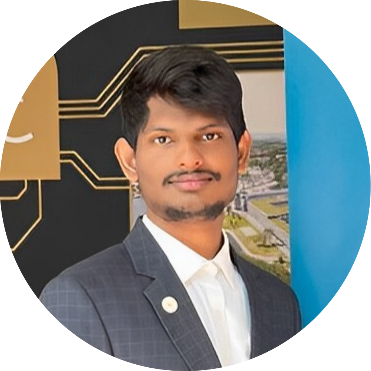
\includegraphics[width=2.7cm,clip]{images/resume_pic_m.png}}
}
\parbox{\dimexpr\linewidth-3.8cm\relax}{
\vspace{-20pt}
\begin{tabularx}{\linewidth}{L r} \\
    {\Huge \scshape  Venkata Sai Yakkshit Reddy Asodi}~
    \href{https://www.cedzlabs.com/yakkshit}{\vspace{1pt}}\\
      Berlin, Germany \\ \vspace{1pt}
     \small \raisebox{-0.1\height}\faPhone\ +91 9493006444 ~ \href{mailto:saiyakkshit2001@gmail.com}{\raisebox{-0.2\height}\faEnvelope\  {saiyakkshit2001@gmail.com}} ~ 
    \href{https://linkedin.com/in/yakkshit/}{\raisebox{-0.2\height}\faLinkedin\ {yakkshit}}  ~
    \href{https://yakkshit.com/}{\raisebox{-0.2\height}\faGlobe\ {yakkshit.com}}  ~
    \href{https://github.com/yakkshit}{\raisebox{-0.2\height}\faGithub{ yakkshit}}
    \vspace{-8pt}
\end{tabularx}
}
\end{center}

\vspace{-23pt}
\href{https://www.yakkshit.com/#details}{\section{Summary \faLink}
Full Stack Developer with 3+ years of experience in both front-end and back-end development. Proven expertise in developing scalable web applications using modern JavaScript frameworks and Python. Strong background in creating responsive user interfaces and implementing robust backend solutions. Demonstrated ability to work effectively in agile team environments while maintaining high code quality and attention to detail.}

\section{\href{https://www.linkedin.com/in/yakkshit/details/skills/}{Technical Skills} \faLink}
\begin{itemize}[leftmargin=0.15in, label={}]
\small{\item{
\textbf{Languages - }{JavaScript (ES6+), Python, Java, HTML5, CSS3, SQL} \\
\textbf{Frontend - }{React.js, Vue.js, Bootstrap, SASS/SCSS, Responsive Design} \\
\textbf{Backend - }{Node.js, Django, RESTful APIs, PostgreSQL, MongoDB} \\
\textbf{DevOps \& Tools - }{Git, Docker, AWS, Jenkins, Agile/Scrum}\\
}}
\end{itemize}
\vspace{-10pt}

\section{Experience \faLinkedin}
\resumeSubHeadingListStart

\resumeSubheading
{\large Circleup AG \faBuilding}{December 2023 -- Present}
{Full Stack Developer}{\faMapMarker \hspace{0.1cm} Zurich, Switzerland}\\
\vspace{10pt}
\textbf{Responsibilities:}
\resumeItemListStart
\vspace{-10pt}
\resumeItem{Developed and maintained full-stack web applications using React.js and Django, resulting in a 40\% improvement in application performance}
\resumeItem{Implemented responsive design principles and CSS best practices, ensuring cross-browser compatibility and mobile-first approach}
\resumeItem{Collaborated with cross-functional teams to design and implement RESTful APIs, improving data processing efficiency by 35\%}
\resumeItemListEnd
\vspace{-3pt}
\textbf{Environment:}\emph{React.js, Django, Python, JavaScript, PostgreSQL, Docker}

\resumeSubheading
{Cedzlabs \faBuilding}{March 2023 -- November 2023}
{Software Developer}{\faMapMarker \hspace{0.1cm} India}\\
\vspace{10pt}
\textbf{Responsibilities:}
\vspace{-10pt}
\resumeItemListStart
\resumeItem{Built and maintained scalable web applications using Java and Spring Boot, serving 10,000+ daily active users}
\resumeItem{Implemented responsive UI components using React.js and Material-UI, reducing page load time by 45\%}
\resumeItemListEnd
\vspace{-3pt}
\textbf{Environment:}\emph{Java, Spring Boot, React.js, MySQL, Git}

\resumeItem{\textbf{\href{https://linkedin.com/in/yakkshit}{Checkout my other experiences by clicking here}}}

\vspace{-5pt}
\section{Projects \faGithub}
\vspace{-5pt}
\resumeSubHeadingListStart
\resumeProjectHeading
{\textbf{\href{https://ui.cedzlabs.com/resume}{E-Commerce Platform}} $|$ \emph{MERN Stack}}{2023}\\
\vspace{6pt}
\textbf{Description:}
\vspace{-5pt}
\resumeItemListStart
\resumeItem{Developed a full-stack e-commerce platform using MongoDB, Express.js, React, and Node.js. Implemented features including user authentication, product catalog, shopping cart, and payment integration. Utilized Redux for state management and implemented responsive design using CSS3 and Bootstrap.}
\resumeItemListEnd
\vspace{4pt}
\textbf{Tools:}\emph{
MongoDB, Express.js, React.js, Node.js, Redux, Bootstrap}
\vspace{-10pt}

\resumeProjectHeading
{\href{https://yakkshit.com}{\textbf{Task Management System}} $|$ \emph{Python, Django, React}}{2023}\\
\vspace{6pt}
\textbf{Description:}
\vspace{-5pt}
\resumeItemListStart
\resumeItem{Created a full-stack task management system with real-time updates using Django REST framework and React. Implemented user authentication, task creation/assignment, and progress tracking features. Deployed using Docker and AWS.}
\resumeItemListEnd
\vspace{4pt}
\textbf{Tools:}\emph{Python, Django, React, PostgreSQL, Docker, AWS}
\vspace{-12pt}

\section{Achievements / Certifications}
\resumeSubHeadingListStart
\resumeItemListStart
\resumeItem{AWS Certified Developer Associate}
\resumeItem{Led a team of 5 developers in implementing a major feature release, completed 2 weeks ahead of schedule}
\resumeItem{Reduced application load time by 50\% through optimization of database queries and frontend caching}
\resumeItemListEnd

\resumeSubHeadingListEnd
\textbf{Strengths:}\emph{Problem-solving, Team collaboration, Technical leadership, Agile methodologies} \\
\textbf{Languages:}\emph{Telugu - Native $|$ English - Fluent $|$ Hindi - Fluent $|$ German - Intermediate}

\vspace{10pt}
\end{document}